The direction vector for $CA$ vector is given by
\begin{align}
\vec{m} &= \vec{A} - \vec{C}\\
&= \myvec{1 \\ -1} - \myvec{-3 \\ -5}\\
&= \myvec{4 \\ 4}
\end{align}
Now, normal vector is given by
\begin{align}
\vec{n} &= \myvec{0&1 \\ -1&0}\vec{m}\\
&= \myvec{0&1 \\ -1&0}\myvec{4 \\ 4}\\
&= \myvec{4 \\ -4}\\
\implies \vec{n}^{\top} &= \myvec{4&-4}
\end{align}
Therefore, normal form of equation of line $CA$ is
\begin{align}
\vec{n}^{\top}(\vec{x} - \vec{C}) &= 0 \\
\implies \vec{n}^{\top}{\vec{x}} - \vec{n}^{\top}{\vec{C}} &= 0 \\
\implies \vec{n}^{\top}{\vec{x}} &= \vec{n}^{\top}{\vec{C}} \\
\implies \myvec{4&-4}{\vec{x}} &= \myvec{4&-4}\myvec{-3 \\ -5} \\
&= -12 + 20 \\
&= 8 
\end{align}
Hence, the required equation of $CA$ is
\begin{align}
\myvec{4&-4}{\vec{x}} &= 8 
\end{align}
\begin{figure}
\centering
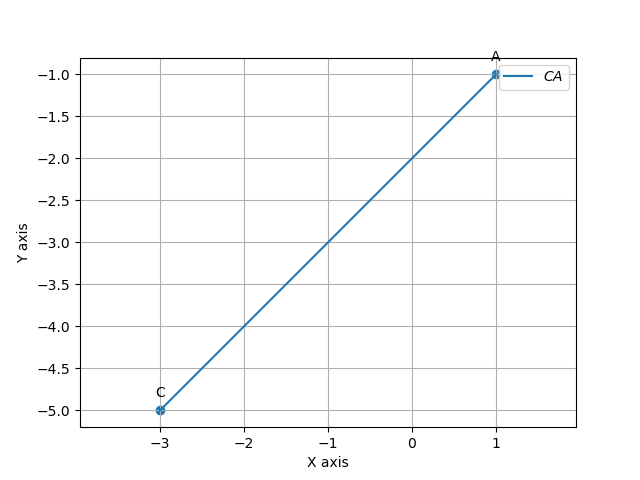
\includegraphics[width=\columnwidth]{solutions/1/1/5c/figs/fig.png}
\caption{Line CA generated using python}
\label{fig: line_CA_py}
\end{figure}

